\documentclass[UTF8]{ctexart}
\usepackage{graphicx}
\usepackage{float}
\usepackage{geometry}
\usepackage{fancyhdr}
\usepackage{lastpage}
\usepackage{enumerate}
\usepackage{multirow}
\usepackage{booktabs}
\usepackage{geometry}
\usepackage{amsmath}
\usepackage{amsthm}
\usepackage{amssymb}
\usepackage{mathrsfs}
\usepackage[linesnumbered,boxed,ruled,commentsnumbered]{algorithm2e}
\geometry{left=2.54cm,right=2.54cm,top=3.18cm,bottom=3.18cm}%页边距
\pagestyle{fancy}
\lhead{
\includegraphics[scale=1]{sjtu-logo-red.pdf}}  
\rhead{BI908 多种方法实现的脑肿瘤分割} 
\cfoot{第 \thepage\ 页\ 共 \pageref{LastPage} 页} 

\begin{document}

\begin{titlepage}
    \begin{center}
        
\includegraphics[width=0.8\textwidth]{sjtu-name-blue.pdf}\\[1cm]
        \textsc{\Huge \bfseries 课程报告}\\[1.5cm]
        
\includegraphics[width=0.3\textwidth]{sjtu-badge-blue.pdf}\\[0.5cm]    

        \Huge \bfseries{BI908 脑肿瘤分割项目报告}\\[1cm]
        \Large \bfseries{518021910971 裴奕博}\\
        \Large \bfseries{518021910795 丁一}\\
        \Large \bfseries{518082910006 陈波}\\
        \Large \bfseries{518021910637 栗行健}
    \end{center}
\end{titlepage}
\tableofcontents
%正文

\newpage
\section{项目简介}
\subsection{项目概述}
本项目采用了阈值分割,区域增长等多种分割算法,结合形态学处理等辅助增强手段,对给定的脑肿瘤进行了分割,并取得了不错的效果。整个项目均采用自己实现的Python算法,项目的总流程如下:
\begin{figure}[H]
    \centering  %图片全局居中
    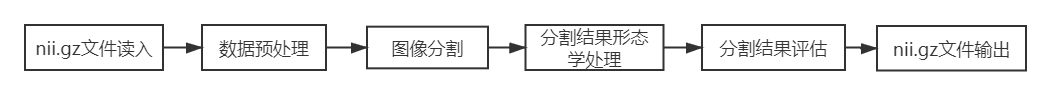
\includegraphics[width=\textwidth]{figure/workflow.png}
    \caption{总工作流程图}
\end{figure}
其中:
% TODO
\begin{enumerate}[1)]
    \item nii.gz文件的输入输出均由SimpleITK包完成
    \item 数据预处理部分的算法包括 % TODO
    \item 图像分割算法包括:去除背景的三维Otsu算法,传统的三维区域增长算法,改进后的三维区域增长算法。
    \item 分割结果的形态学后处理方法包括:开运算和闭运算操作。
\end{enumerate}

\subsection{采用数据}
我们组的编号为04,采用的数据集是Dataset\_Group/04文件夹下的三个待分割样本,编号分别为$BRAT\_008,BRAT\_033,BRAT\_259$。


\subsection{各文件(夹)功能}
\begin{itemize}
    \item README.md文件:说明了本项目的主要信息和使用方法。
    \item requirements.txt文件:说明了本项目所需环境中的依赖包。
    \item Dataset\_Group文件夹:存放待分割样本和标签。
    \item train\_data文件夹:存放经切片之后的二维图像,可供深度学习使用。
    \item output文件夹:存放经过算法之后输出的文件,文件夹下共由5个子文件夹,对应5种分割和结果后处理的方法。
    \item run.bat文件:命令行运行脚本,用户若需要再不同的分割方式下进行切换,可以直接在该文件中修改参数实现。
    \item main.py文件:整个项目的主函数,包含了从数据读入,调用算法和结果评估,输出结果的全过程。
    \item iotest.py/sitk\_test.py/iotest.nii.gz文件:项目实现过程中的调试文件和调试输出,用户使用时不要运行。
    \item prepare.py文件:用于将原始数据切片并上采样至256$\times$256的二维图像,其结果输出为jpg格式,存放在train\_data文件夹中。
    \item otsu.py文件:实现了三维的Otsu阈值分割函数。
    \item region\_growing.py文件:实现了三维的区域增长分割函数。
    \item validation.py文件:实现了混淆矩阵(confusion matrix)和所有评价指标的求取。
    \item visualize.py文件:输出分割的可视化结果。
    \item config.py文件:存放算法过程中所需的常量。
    \item utils.py文件:实现算法过程中其余所有需要用到的辅助函数(如输入输出、可视化、形态学算法等)
    \item result.json文件:存放分割算法的评价指标原始数据。
    \item result\_to\_csv.py文件:将json中的原始数据读出后转换并整理为csv格式。
    \item result.csv文件:存放本项目各方法的最终对比结果。
\end{itemize}

\subsection{使用说明}
见README.md文件中run部分。

\section{实现思路与方法}
\subsection{基于多阈值Otsu的图像分割}
从数据集和标签的对比中我们可以看到,脑肿瘤对应的区域基本为原图的高亮区,与周围组织灰度相差较大,因此最简单直接的思路就是考虑直接通过阈值处理进行分割,由于要自动选择阈值,因此我们采用了Otsu算法,并将其扩展至三维。

\subsubsection{传统的多阈值Otsu方法}
传统二阈值Otsu算法的基本假设如下:假定图像包含几类像素,直方图为多峰直方图,然后计算使得多类像素能分开的最佳阈值(类内方差),或等价的间类间方差最大。

写成伪代码将思路表示如下:

\begin{algorithm}[H]
    \caption{Traditional Otsu}\label{algorithm}
    \KwIn{img: 3d-array of size $w\times h\times q$}
    \KwOut{result,t1,t2}
        Initialize t1,t2,result\;
        $m_g$=mean(img)\;
        \For {t1 = 0 to GRAY\_MAX}{
            \For{t2 = 1 GRAY\_MAX-1}{
                m1=mean(img[img<t1])\;
                p1=count(img[img<t1])\;
                m2=mean(img[img>t1 and img<t2])\;
                p2=count(img[img>t1 and img<t2])\;
                m3=mean(img[img>t2])\;
                p3=count(img[img>t2])\;
                var[t1][t2]=$p1*(m1-m_g)^2+p2*(m2-m_g)^2+p3*(m3-m_g)^2$\;
            }
        }
        t1,t2=argmax(var)\;
        result=img[img>t2]\;
        \Return{result,t1,t2}
        
\end{algorithm}

	t1,t2即为所求。Otsu方法可以形象地理解为:求取直方图多个峰值之间的低谷值t1,t2。
\subsubsection{改进后的Otsu方法}
使用传统的Otsu算法之后,发现对部分样本效果不佳,原因是在整个三维图像中,背景像素(即灰度值接近0的像素)过多,也输出了很多噪点,导致最后输出的结果不佳。因此我们对传统的Otsu算法进行了一下几点改进:
\subsubsection*{阈值与背景处理}
经过改进,我们将所有灰度值小于某阈值t(实际取值为10)的像素点忽略,不计入均值和方差的计算中。这一改进既提升了算法的速度,又避免了大面积背景的影响。


\subsubsection*{添加形态学后处理}
仅用上述改进的otsu代码分割肿瘤时出现了两处问题:
\begin{itemize}
    \item 肿瘤外部有独立小分区(来源于图像的独立高亮噪点)。
    \item 肿瘤内部出现未闭合区域(来源于原图像肿瘤区域中的暗区)。
\end{itemize}

为了有效避免这两种情况的出现,我们对解雇采取了形态学操作的后处理方法,采用了先闭运算后开运算的方法。闭运算→开运算:闭运算(先膨胀再腐蚀)可以填平小孔,弥补小裂缝,并保持总的位置和形状不变;开运算(先腐蚀再膨胀)可以去除孤立小点,毛刺和小桥,总的位置形状不变。故结合闭运算和开运算进行预处理,有效避免了直接otsu处理所产生的两处问题,提高了分割的有效性。

\subsubsection*{同直接遍历对比}

直接遍历图像得到能够用于分割图像的阈值点,一般用手动选择的方式确定分割阈值,从算法复杂度看,直接遍历和otsu是相同的,但是由于otsu可以自动选择合适的阈值且有合理的数学依据,相比直接遍历的人工选择有着巨大的优势。

\subsubsection*{改进后的算法}
经过以上几点改进,我们的算法思路可以表示如下:

\begin{algorithm}[H]
    \caption{Our new Otsu}\label{algorithm}
    \KwIn{img: 3d-array of size $w\times h\times q$, t:int}
    \KwOut{result,t1,t2}
        Initialize t1,t2,result\;
        $m_g$=mean(img)\;
        \For {t1 = t+1 to GRAY\_MAX}{
            \For{t2 = t+2 GRAY\_MAX-1}{
                m1=mean(img[img<t1 and img>t])\;
                p1=count(img[img<t1 and img>t])\;
                m2=mean(img[img>t1 and img<t2])\;
                p2=count(img[img>t1 and img<t2])\;
                m3=mean(img[img>t2])\;
                p3=count(img[img>t2])\;
                var[t1][t2]=$p1*(m1-m_g)^2+p2*(m2-m_g)^2+p3*(m3-m_g)^2$\;
            }
        }
        t1,t2=argmax(var)\;
        result=img[img>t2]\;
        result=opening(closing(result))\;
        \Return{result}
        
        
\end{algorithm}

\subsubsection{otsu算法总结}

	我们使用的三维otsu算法从最终结果上看是符合要求的,最初我们有想通过分割成155张二维图像分别进行otsu处理(其结果与三维处理相同),但是这是间接进行分割,在实际应用中可能会碰到繁冗步骤与分割的不确定性,故改写otsu算法可以对三维图像进行直接处理,由于去除了背景,大大降低了运算时间并提高了阈值的准确度。为了更好地分割图像,我们去除了背景,添加了闭运算与开运算进行后处理,去除了孤立区域(亮点与暗点)。整体而言,otsu算法在此类有着较为明显区间阈值差异图像中有很好的体现,但是缺陷比较明显,在肿瘤区域高亮时容易分割,区域高亮但是有明显灰度值差异如800和1000左右的差异,会导致阈值的选取出现异常,出现较大的暗区或者分割部分变小。正因如此,我们考虑到了区域增长的办法进行图像分割。




\subsection{基于区域增长的图像分割}
\subsubsection{传统的区域增长方法}
区域生长是根据事先定义的准则将像素或者子区域聚合成更大区域的过程。其基本思想是从一组生长点开始(生长点可以是单个像素,也可以是某个小区域),将与该生长点性质相似的相邻像素或者区域与生长点合并,形成新的生长点,重复此过程直到不能生长为止。生长点和相似区域的相似性判断依据可以是灰度值、纹理、颜色等图像信息。所以区域生长算法关键有三个:
\begin{itemize}
    \item 选择合适的生长点
	\item 确定相似性准则即生长准则
	\item 确定生长停止条件
\end{itemize}
根据输入图像,我们同样将其扩展至三维,传统的区域增长方法可以表示如下:

\begin{algorithm}[H]
	\caption{Traditional region growing}\label{algorithm}
    \KwIn{img: 3d-array of size $w\times h\times q$,seed: list of len=3, radius:int, t:int}
    \KwOut{ifsearch}	
    Initialize ifsearch,head,tail,region\_queue\;
    \While{head<tail}{
        center=region\_queue.pop()\;
        head++\;
        \ForAll{point in distance(point,center)<radius}{
            \If{abs(img[point]-img[center]<t)}{
                ifsearch[point]= 1\;
                region\_queue.push(point)\;
                tail++\;
            }
        }
    } 
    
    \Return{ifsearch}
\end{algorithm}

\subsubsection{改进后的区域增长方法}
在区域增长算法的使用过程中,我们发现了各种问题,比如在有些样本中,区域很难向外生长,而在另一部分样本中,增长的区域与正常脑组织混杂难以收敛,区域出现空洞等各种问题,因此我们对传统的区域增长方法也加以了几点小小的改进。

    \subsubsection*{高亮区域分割的去绝对值处理}

    区域增长的传统判定标准是abs(img[point]-img[center]<t),我们按照这个思路进行分割时会出现区域难以增长的现象,这是因为肿瘤高亮部分会有一部分灰度值过大,在区域增长中被排除在外(在样本中出现了只增长几十个点的情况)。故改进后的算法去掉了abs,即将所有大于邻域中心灰度值的点都采纳,这样肿瘤中高亮部分能够全部被囊括,能够提高统计学的有效性判断。
    \subsubsection*{闭运算后处理}

    由于肿瘤区域存在部分暗区或者孤立暗点,故利用闭运算的方式来填充孔洞,弥补缝隙,使得增长区域更加完整。但由于在区域增长中,增长区域连续的程度显然比用阈值处理的结果高得多,因此这一后处理的效果在不同样本上体现的效果也有较大差异。

    \subsubsection*{强制终止迭代}

    在代码调试阶段,由于阈值和种子点选取不同,有时会导致区域增长出现越界现象,即将整个脑区增长完,同肿瘤区的几万个点相比,脑区总点数超过百万,故我们设定了强制终止点,当生长开始后所判断符合要求的点数超过终止数时停止生长。这样做可以在一定程度上能够限定区域增长总是在肿瘤区附近,不会出现增长区域扩散至整个脑区的现象。这一改进对于肿瘤在某个方向上与脑区界限比较模糊的状况有着良好的效果。

    \subsubsection*{改进后的算法}
    
    \begin{algorithm}[H]
        \caption{Our new region growing}\label{algorithm}
        \KwIn{img: 3d-array of size $w\times h\times q$,seed: list of len=3, radius:int, t:int,tailmax:int}
        \KwOut{ifsearch}	
        Initialize ifsearch,head,tail,region\_queue\;
        \While{head<tail}{
            \If{tail>tailmax}{
                break\;
            }
            center=region\_queue.pop()\;
            head++\;
            \ForAll{point in distance(point,center)<radius}{
                \If{img[point]-img[center]>t}{
                    ifsearch[point]= 1\;
                    region\_queue.push(point)\;
                    tail++\;
                }
            }
        }
        \For{i =head to tail}{
            ifsearch[region\_queue[i]]=1
        }
        ifsearch=closing(ifsearch)
        \Return{ifsearch}
    \end{algorithm}


    \subsubsection{与otsu算法对比}

    在我们选用的样本中,区域增长和ostu算法各有优劣,从算法原理上看,区域增长更适合作为分割肿瘤的处理手段,不过由于医学图像肿瘤区的高亮特性,利用otsu算法也能够得到比较好的结果。区域增长由于可以不断调整参数,能够人为的提高分割的准确性,在医学分割领域有更好的前景。

    \subsubsection{区域增长算法总结}

	区域增长在设计好各项参数后,能够得到比其余分割算法更好的结果。在医学图像中,肿瘤一般具有高亮且边缘明显的特征,利用区域增长处理图象时,要么得到肿瘤区域,要么得到非肿瘤区域,这两种结果都可以有效分割出期望结果。但是由于区域增长原理,有时会出现过度增长甚至全局增长的结果,此时需要进行图像预处理或人工参数设定与代码优化。总体而言,区域增长在医学领域有着较好的应用前景。



\section{项目评价}
\subsection{各方法效果比较}
% Table generated by Excel2LaTeX from sheet 'result'
\begin{table}[H]
    \centering
    \caption{各方法效果评价对照表}
      \begin{tabular}{clrrrrr}
        \toprule
      \multicolumn{1}{l}{sample\_name} & method & \multicolumn{1}{l}{sensitivity} & \multicolumn{1}{l}{precision} & \multicolumn{1}{l}{iou} & \multicolumn{1}{l}{dice} & \multicolumn{1}{l}{time\_cost(s)} \\
            \midrule
      \multirow{5}[0]{*}{BRATS\_008} & multi-threshold Otsu & 0.765708 & 0.934346 & 0.726613 & 0.841663 & 46.87496 \\
            & Otsu\_with\_opening\_closing & 0.836849 & 0.969602 & 0.815455 & 0.898348 & 109.2742 \\
            & traditional\_region\_growing & 0.690839 & 0.885097 & 0.633981 & 0.775996 & 32.8455 \\
            & new\_region\_growing & 0.771337 & 0.988272 & 0.764341 & 0.866432 & 31.56555 \\
            & new\_region\_growing\_closing & 0.86502 & 0.973434 & 0.84507 & 0.916031 & 75.57341 \\
      \multirow{5}[0]{*}{BRATS\_033} & multi-threshold Otsu & 0.742815 & 0.799434 & 0.626128 & 0.770085 & 46.88871 \\
            & Otsu\_with\_opening\_closing & 0.821778 & 0.938875 & 0.780044 & 0.876432 & 108.9621 \\
            & traditional\_region\_growing & 0.726808 & 0.66507 & 0.532062 & 0.694569 & 26.09956 \\
            & new\_region\_growing & 0.90838 & 0.831212 & 0.766916 & 0.868085 & 25.88579 \\
            & new\_region\_growing\_closing & 0.963514 & 0.754597 & 0.733633 & 0.846354 & 68.7768 \\
      \multirow{5}[0]{*}{BRATS\_259} & multi-threshold Otsu & 0.770203 & 0.801038 & 0.646522 & 0.785318 & 46.12582 \\
            & Otsu\_with\_opening\_closing & 0.785546 & 0.733511 & 0.611133 & 0.758637 & 114.2537 \\
            & traditional\_region\_growing & 0.00024 & 1     & 0.00024 & 0.00048 & 0.755245 \\
            & new\_region\_growing & 0.811385 & 0.996561 & 0.80912 & 0.89449 & 10.63574 \\
            & new\_region\_growing\_closing & 0.853095 & 0.994516 & 0.849101 & 0.918393 & 53.55093 \\
            \bottomrule
      \end{tabular}%
    \label{tab:addlabel}%
  \end{table}%  
  
  \begin{figure}[H]
    \centering  %图片全局居中
    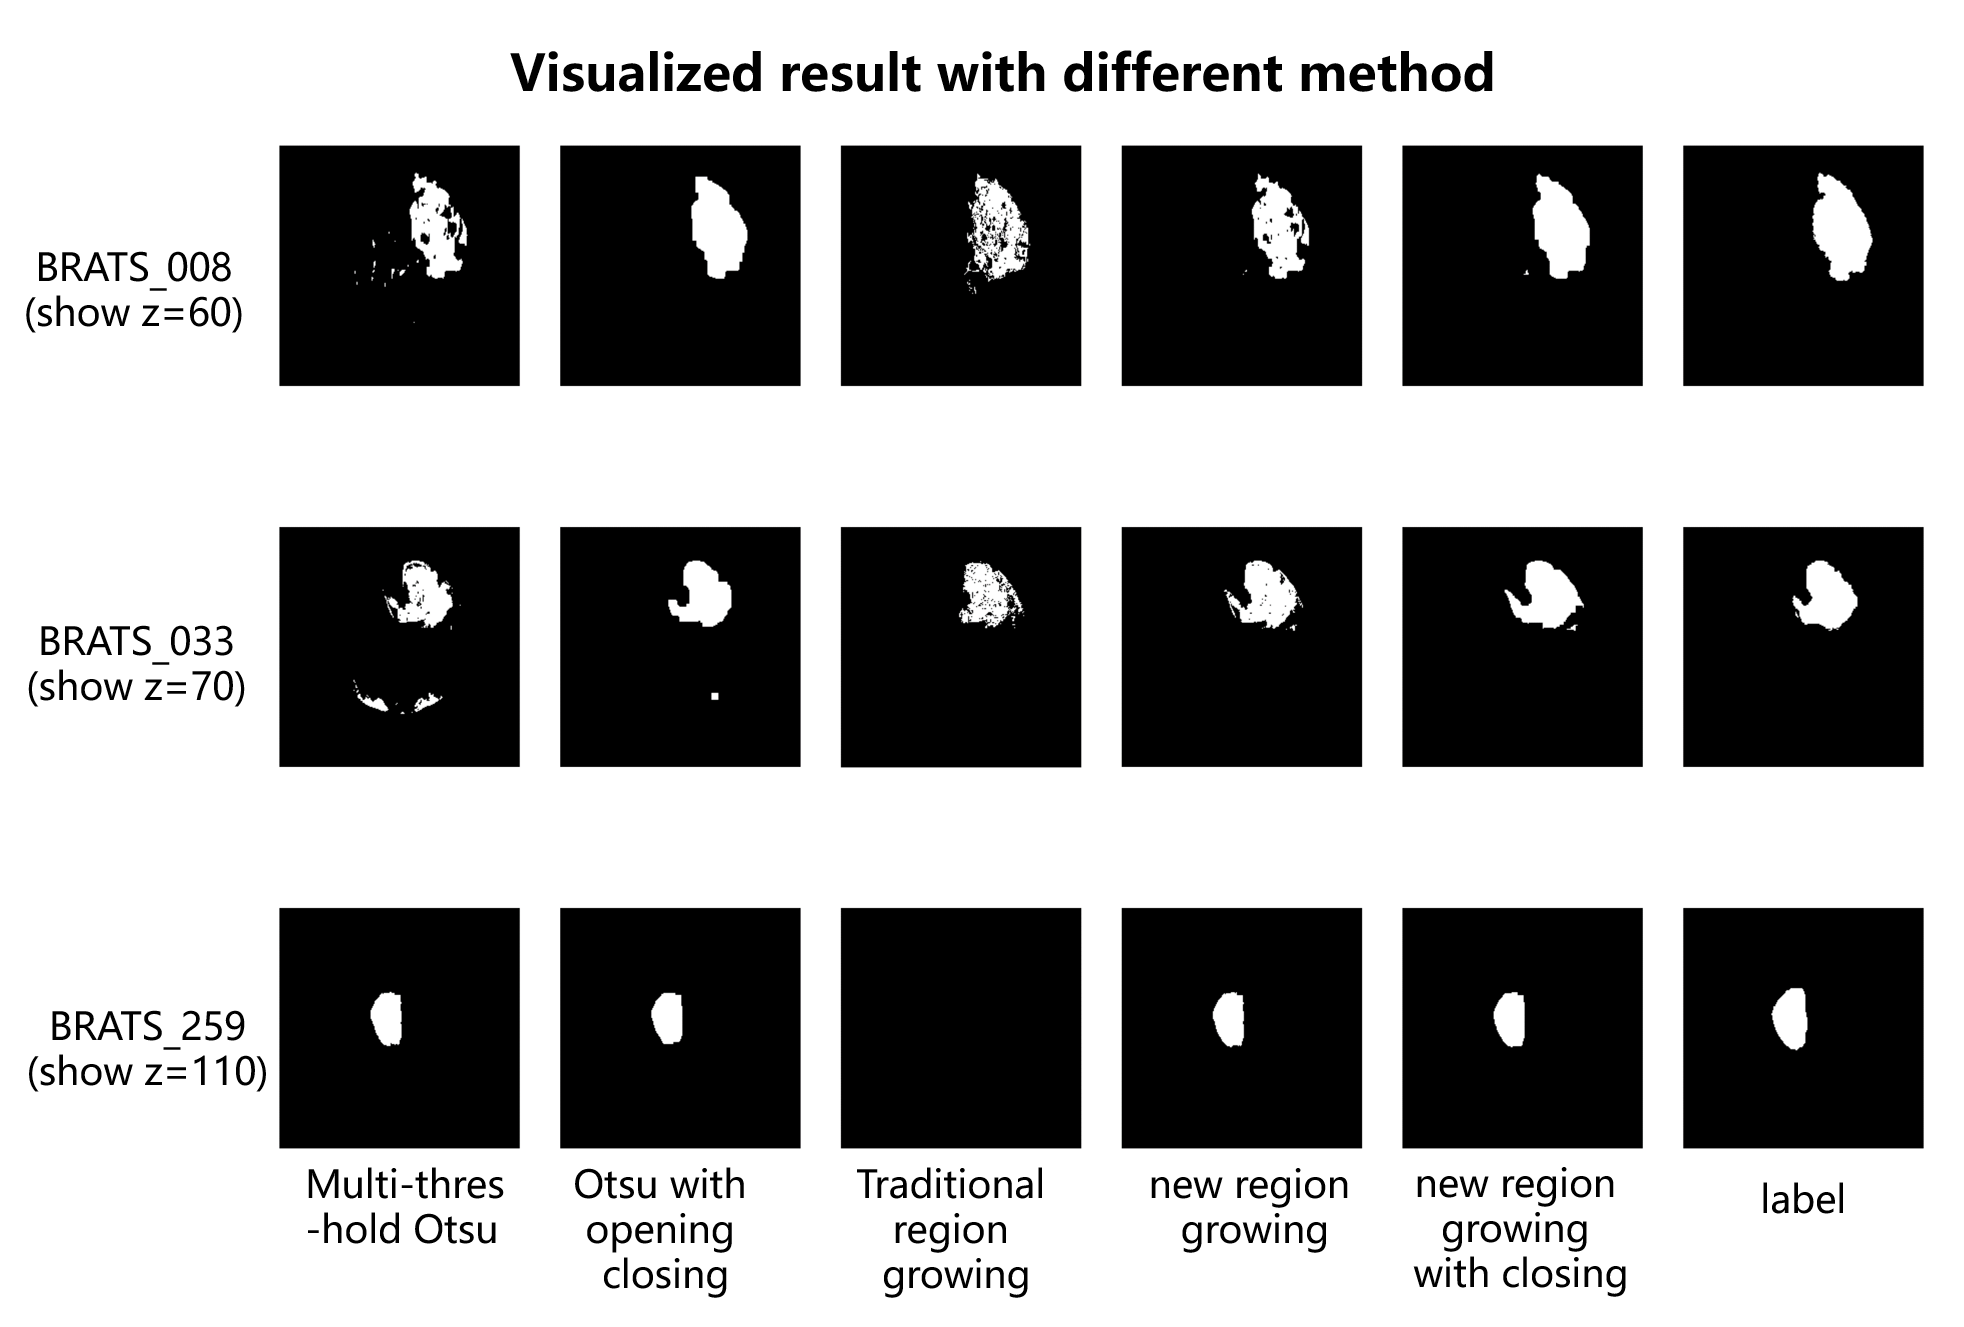
\includegraphics[width=\textwidth]{figure/result.png}
    \caption{各方法可视化对比}
\end{figure}

\subsection{项目优势}
\subsection{项目不足}

\section{成员分工与贡献}
\subsection{裴奕博}
\begin{itemize}
    \item 完成了输入输出、可视化、结果评估、运行脚本等辅助函数的实现。
    \item 与组内其他成员共同讨论,提出了分割算法改进的思路。
    \item 完成了后续说明文档的书写,并与组内其他成员共同完成了项目报告。
\end{itemize}
\subsection{丁一}
\subsection{陈波}
\subsection{栗行健}

\section{感想与展望}
	
	\subsection{项目感想与评价}

	本小组使用了region growing和Otsu两种方法来对脑部肿瘤进行分割,并且在原有算法的基础上进行了一些改进,同时对于算法进行了封装,使得该算法在操作简单的同时,结果实现了更高的准确率。下面给出IoU的评价指标:

	$$ IoU <{0.5} : Poor $$
	$$ {0.5}<IoU<{0.8} : Great $$
	$$ IoU>{0.8} : Excellent $$

	可见我们设计的分割算法已经达到了非常好的效果。但是它们仍然具有一定的局限性。其中最为显著的两个缺点是:

	1.局限性高,尽管每个样本的肿瘤区域都以高亮部分显示,但它们的位置和灰度仍有着区别。这意味着我们在对于每一个肿瘤组织进行区域增长分割时,都需要通过多次尝试种子的点来找到最适合的起始点。此外对于Otsu算法,可能也需要更改舍弃的黑色背景大小来提高精度。

	2.算法复杂度高,在算法中使用了多个for循环嵌套,使得算法拥有很高的时间复杂度。每一种方法的运算时间可能达到了30s。在需要批量处理的场合,这样的时间复杂度是不可取的。

	于是,我们希望对于算法进行进一步的改进,使得它能够更好地应用于实际生活中,碍于时间和能力,仅以理论展示如下改进想法:

	\subsection{未来展望}

	\subsubsection{GPU加速算法}

	\subsubsection*{GPU架构介绍}

    图形处理单元(Graphics Processing Unit,GPU)是由NVIDIA公司于1999年起开发的专门用于计算机图形处理的处理器。它的处理器架构与传统的CPU有很大的差别。GPU主要以负责计算任务的执行单元以及存储器单元为主。
    
    \begin{figure}[H]
        \centering  %图片全局居中
        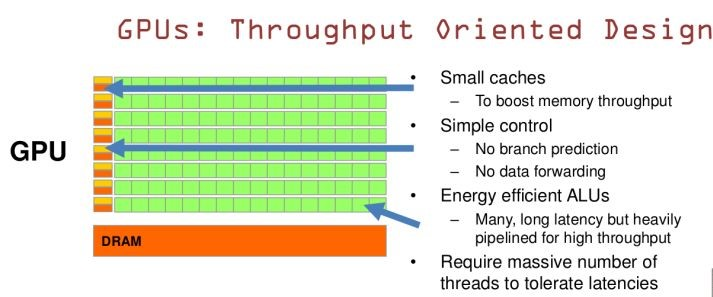
\includegraphics[scale=0.4]{figure/Gpu structure.jpg}
        \caption{GPU并行计算}
    \end{figure}

	与CPU擅长逻辑控制,串行的运算。和通用类型数据运算不同,GPU擅长的是大规模并发计算,如本算法中计算量大但简单的工作,因此可以设计GPU加速算法应用于本文的工作.
	
	\subsubsection{自动寻找种子算法设计}

	可以设计一个算法,自动寻找到三维图像中高亮像素点密集的区域,并生成一个三维的模型,通过选取模型的中间像素点,得到我们所需要的种子值。

	为了提高分割的精度,我们也可以通过对该点附近的多个点进行区域生长计算,取其中精度最高的点来作为我们得到的模型,注意到该算法实际上大大增加了时间上的消耗,但它为自动化区域增长分割算法提供了一种思路,此外,通过并行化GPU加速算法的设计与使用,也使得这种设想成为了一种可能。

	\subsection{总结和致谢}

    通过本学期的课程,我们学习到了很多关于图像处理的知识,而本次的大作业也是对我们所学知识的一次检测。在实现本次大作业的过程中,我们既感受到了图像处理的神奇,为所得到的结果而激动,同时也在查阅资料的过程中感受到了自己所学知识的不足,本学期所学的知识仅仅是冰山一角,图像需要我们进一步地深入学习,“路漫漫其修远兮,我将上下而求索。”
    
    最后,感谢老师和助教在本次大作业中给予我们的帮助的解答!

\end{document}
